\documentclass{gtpart}
\usepackage{amsmath,amssymb,amsthm,stmaryrd}
\usepackage[all]{xy}
\usepackage{tikz}
\usepackage{url}
\usepackage{hyperref}
\usepackage{enumerate}
\usepackage{tensor}
%/home/grad/zyf/TeX/inputs/
\usepackage{mathrsfs}
%\usepackage{mathpazo}
%\usepackage[mathpazo]{flexisym}
%\usepackage{breqn}
%\usepackage{amsrefs}
%\usepackage{setspace}
%\doublespacing

\title{The power operation structure on Morava $E$-theory of height 2 at the prime 3}
\author{Yifei Zhu}
\givenname{Yifei}
\surname{Zhu}
\address{Department of Mathematics\\University of Minnesota\\Minneapolis, MN 55455\\USA}
\email{zyf@math.umn.edu}

%\subject{primary}{msc2000}{55P99}
%\subject{secondary}{msc2000}{55Q99}

%\bibliographystyle{gtart}
\parskip 0.7pc
\parindent 0pt

\newtheorem{thm}{Theorem}
\newtheorem{cor}[thm]{Corollary}
\newtheorem{prop}[thm]{Proposition}
\newtheorem{lem}[thm]{Lemma}
\theoremstyle{definition}
\newtheorem{defn}[thm]{Definition}
\theoremstyle{remark}
\newtheorem{rmk}[thm]{Remark}
\newtheorem{exam}[thm]{Example}
\newtheorem{case}[thm]{Case}
\newtheorem{slogan}[thm]{Slogan}
\newtheorem{ques}[thm]{Question}

\def\co{\colon\thinspace}
\newcommand{\mb}[1]{\mathbb{#1}}
\newcommand{\mf}[1]{\mathfrak{#1}}

\newcommand{\NB}[1]{{\bf (NB: #1)}}

\newcommand{\Ext}{\ensuremath{{\rm Ext}}}
\newcommand{\Coext}{\ensuremath{{\rm Coext}}}
\newcommand{\Hom}{\ensuremath{{\rm Hom}}}
\newcommand{\Tor}{\ensuremath{{\rm Tor}}}
\newcommand{\Ind}{\ensuremath{{\rm Ind}}}
\newcommand{\Res}{\ensuremath{{\rm Res}}}
\newcommand{\colim}{\ensuremath{\mathop{\rm colim}}}
\newcommand{\hocolim}{\ensuremath{\mathop{\rm hocolim}}}
\newcommand{\holim}{\ensuremath{\mathop{\rm holim}}}
\newcommand{\overto}{\mathop\rightarrow}
\newcommand{\overfrom}{\mathop\leftarrow}
\newcommand{\into}{\mathop\hookrightarrow}
\newcommand{\onto}{\mathop\twoheadrightarrow}
\newcommand{\longoverto}{\mathop{\longrightarrow}}
\newcommand{\Irr}{\ensuremath{\mathop{\rm Irr}}}
\newcommand{\Rep}{\ensuremath{\mathop{\rm Rep}}}
\newcommand{\Map}{\ensuremath{{\rm Map}}}
\newcommand{\GL}{{\rm GL}}
\newcommand{\Uni}{{\rm U}}
\newcommand{\BU}{{\rm BU}}
\newcommand{\Sp}{{\cal S}p}
\newcommand{\Sym}{{\rm Sym}}
\newcommand{\thh}{{\rm thh}}
\newcommand{\TAF}{{\rm TAF}}
\newcommand{\TAQ}{{\rm TAQ}}
\newcommand{\End}{{\rm End}}
\newcommand{\Aut}{{\rm Aut}}
\newcommand{\As}{{\cal A}s}
\newcommand{\LT}{{\rm LT}}
\newcommand{\Spec}{{\rm Spec\thinspace}}
\newcommand{\Spf}{{\rm Spf}}
\newcommand{\tmf}{{\rm tmf}}
\newcommand{\eo}{{\rm eo}}
\newcommand{\TMF}{{\rm TMF}}
\newcommand{\Ell}{{\cal E}ll}
\newcommand{\Lie}{{\rm Lie}}
\newcommand{\Sh}{{\rm Sh}}
\newcommand{\HF}{{\rm H}{\mb F}}
\newcommand{\cF}{\overline {\mb F}}
\newcommand{\cQ}{\overline {\mb Q}}

\newcommand{\eilm}[1]{\ensuremath{{\mb H} #1}}
\newcommand{\smsh}[1]{\ensuremath{\mathop{\wedge}_{#1}}}
\newcommand{\tens}[1]{\ensuremath{\mathop{\otimes}_{#1}}}
\newcommand{\susp}{\ensuremath{\Sigma}}
\newcommand{\mapset}[3]{\ensuremath{\left[#2,#3\right]_{#1}}}
\newcommand{\form}[2]{\ensuremath{\left\langle#1,#2\right\rangle}}
\newcommand{\bilin}[2]{\ensuremath{\left(#1,#2\right)}}
\newcommand{\comp}[1]{\ensuremath{#1^\wedge}}
\newcommand{\loca}[3]{\ensuremath{L^{#1}_{#2}(#3)}}
\newcommand{\tc}[3]{\ensuremath{\Omega_{#2 / #1}^{#3}}}
\newcommand{\atc}[3]{\ensuremath{\L_{#2 / #1}^{#3}}}

\newcommand{\xym}[1]{
\vskip 0.7pc
\centerline{\xymatrix{#1}}
\vskip 0.7pc
}

%\newcommand{\DL}{{\rm DL}}
\newcommand{\CA}{{\cal A}}
\newcommand{\Mod}{{\rm Mod}}
\newcommand{\Alg}{{\rm Alg}}
\newcommand{\Frob}{{\rm Frob}}
\newcommand{\DF}{{{\rm DefFrob}_\Gamma}}
\newcommand{\Model}{{\rm Model}}
\newcommand{\Gm}{{{\mb G}_m}}
\newcommand*{\longhookrightarrow}{\ensuremath{\lhook\joinrel\relbar\joinrel\rightarrow}}
\newcommand{\cf}[1]{cf.\thinspace{\cite{#1}}}
\newcommand{\cff}[2]{cf.\thinspace{\cite[#1]{#2}}}

\usepackage{mathtools}

\newcommand{\DL}{Dyer--Lashof~}
\newcommand{\BF}{{\mb F}}
\newcommand{\BP}{{\mb P}}
\newcommand{\BZ}{{\mb Z}}
\newcommand{\CM}{{\mathscr{M}}}
\newcommand{\HC}{\widehat{C}}
\newcommand{\HS}{\widehat{S}}
\newcommand{\TG}{\widetilde{\G}}
\newcommand{\Tf}{\widetilde{f}}
\newcommand{\TP}{\widetilde{\psi}}
\newcommand{\md}{~~{\rm mod}~}
\newcommand{\A}{\alpha}
\newcommand{\p}{\psi^3}
\newcommand{\G}{\Gamma}
\newcommand{\s}{S_{3,3}}
\newcommand{\CO}{{\mathscr{O}}}

\begin{document}
\begin{abstract}
 We give explicit calculations of the algebraic theory of power operations for a specific Morava $E$-theory spectrum and its $K(1)$-localization.  
 At height 2 for the prime 3, the power operations arise from the universal degree-3 isogeny of elliptic curves associated to the $E$-theory.  
\end{abstract}


\maketitle
\section{Introduction}
\label{sec:intro}

The study of cohomology operations has been central to algebraic topology 
since the 1950s, with applications to solving problems such as the number of independent vector fields 
on spheres, and the non-existence of maps of Hopf invariant one.  
Perhaps internally cohomology operations are primarily used to cure the blindness of cohomology theories \cite{blind}, 
that is, to cure their varied degrees of inability to detect the fact that a map of spaces is essential.  

Suppose $E$ is a commutative $S$-algebra, in the sense of \cite{EKMM}, and $A$ is a commutative $E$-algebra.  
We want to capture the properties and underlying structure of the homotopy groups $\pi_* A = A_*$ of $A$, 
by studying operations associated to the cohomology theory that $E$ represents.  

An important family of cohomology operations, called {\em power operations}, is constructed via the extended powers.  
Specifically, consider the functor of {\em the $m$th extended power over $E$} from the category of $E$-modules to the category of commutative $E$-algebras 
\[
 \BP_E^m (-) \coloneqq (-)^{\wedge_E m} / \Sigma_m \co \Mod_E \to \Alg_E 
\]
which sends an $E$-module to its $m$-fold smash product over $E$ modulo the action by the symmetric group on $m$ letters.  
The $\BP_E^m (-)$'s assemble together to give the {\em free commutative $E$-algebra functor} 
\[
 \BP_E (-) \coloneqq \bigvee_{m \geq 0} \BP_E^m (-) \co \Mod_E \to \Alg_E.  
\]
These functors descend to homotopy categories.  
In particular, each $\A \in \pi_{d+i}~\BP_E^m (\Sigma^d E)$ gives rise to a power operation 
\[
 Q_\A \co A_d \to A_{d+i} 
\]
(\cff{Sections I.2 and IX.1}{H_infty} and \cite[Section 3]{cong}).  

Under the action of power operations, $A_*$ is an algebra over some operad on $E_*$-modules involving the structure of $E_* B\Sigma_m$ for all $m$.  
This operad is traditionally called a {\em \DL algebra}, or more precisely, 
a \DL {\em theory} as the {\em algebraic theory} of power operations acting on the homotopy groups of commutative $E$-algebras 
(\cff{Chapters III, VIII, and IX}{H_infty} and \cite[Section 9]{lpo}).  

A specific case is when $A$ is $K(n)$-local and $E$ is a Morava $E$-theory of height $n$.  
Morava $E$-theory spectra are of crucial importance in modern stable homotopy theory, 
particularly in the work of Ando, Hopkins, and Strickland \cite{cube}.  
Much of the $K(n)$-local $E$-\DL theory has been worked out by those authors (\cff{1.5}{cong} for a description of the history).  
In \cite{cong} Rezk gives a unified treatment of this \DL theory.  
He works out a congruence criterion that must hold in an algebra over the \DL theory (\cite[Theorem A]{cong}).  
This enables one to study the \DL {\em theory}, which models all the algebraic structure naturally adhering to $A_*$, 
by working with a certain associative ring $\G$ as the \DL {\em algebra}.  
Moreover, Rezk provides a geometric description of this congruence criterion, 
in terms of sheaves on the moduli problem of deformations of formal groups and Frobenius isogenies (\cff{Theorem B}{cong}).  
This connects the structure of $\G$ to the geometry underlying $E$, 
moving one step forward from a workable object $\G$ to something computable.  
Based on these, in a companion paper \cite{h2p2}, 
Rezk gives explicit calculations of the \DL theory for a specific Morava $E$-theory of height $n = 2$ at the prime 2.  

The purpose of this paper is to make available calculations analogous to some of the results in \cite{h2p2}, at the prime 3, 
together with calculations of the corresponding $K(1)$-local power operations.  


\subsection*{Outline of the paper}

As in \cite{h2p2}, the computation of power operations in this paper follows the approach of \cite{steenrod}: 
one first defines a total power operation, 
and then uses the computation of the cohomology of the classifying space of the symmetric group $\Sigma_m$ to obtain individual power operations.  
These two steps are carried out in Sections \ref{sec:psi} and \ref{sec:Gamma} respectively.  

In Section \ref{sec:psi}, by doing calculations with a specific elliptic curve associated to our Morava $E$-theory $E$, 
we give formulas of the total power operation $\p$ on $E_0$ and the ring $S_3$ parametrizing the corresponding moduli problem.  

In Section \ref{sec:Gamma}, based on calculations of $E_* B\Sigma_m$ in \cite{Str98}, 
we define individual power operations, and derive the relations they satisfy.  
Thus in view of the general structures described in \cite{cong}, 
we get an explicit description of the \DL algebra $\G$ for $K(2)$-local commutative $E$-algebras.  

In Section \ref{sec:K(1)}, we describe the relationship between the total power operation $\p$, at height 2, and the corresponding $K(1)$-local power operation.  
We then derive formulas of the latter from the calculations in Section \ref{sec:psi}.  

In Appendices \ref{apx:tors} and \ref{apx:isog}, we list long formulas whose appearance in the main body might affect readability.  

\begin{rmk}
 The ring $S_3$ mentioned above turns out to be an algebra on one generator over the base ring where our elliptic curve is defined 
 (cf.\thinspace{P}roposition \ref{prop:isog}).  This generator appears as a parameter in the formulas of the total power operation $\p$, 
 and is responsible for how the individual power operations are defined and how their formulas look.  
 Different choices of this parameter results in different bases of the \DL algebra $\G$.  

 The parameter in this paper will be derived differently from the one used in \cite{h2p2}; 
 it comes intrinsically from the relative cotangent space of the elliptic curve at the identity.  
 This choice of parameter is important for writing down Adem relations in Section \ref{sec:Gamma}, 
 and it fits naturally into the treatment of gradings in \cite{cong}.  

 We should point out that our choice is by no means canonical; 
 we do not know yet, as part of the structure of the \DL algebra, 
 if there is a {\em canonical} basis which is both geometrically interesting and computationally convenient.  
 Somewhat surprisingly, although it appears to come from different considerations, 
 our choice has an analog at the prime 2 which coincides with the parameter used in \cite{h2p2}.  
 Our calculations follow a recipe in hope of generalizing to other Morava $E$-theories at height 2; 
 we hope to address these matters and recognize more of the general patterns based on further computational evidence.  
\end{rmk}


\subsection*{Acknowledgements}

I thank Charles Rezk for encouragement on this work, and for his observation in a correspondence which led to Proposition \ref{prop:-p} and Corollary \ref{cor:-p}.  
I thank Tyler Lawson for the sustained support from him I received as a student.  


\subsection*{Conventions}

Let $p$ be a prime, $q$ a power of $p$, and $n$ a positive integer.  We use the symbols 
\[
 \BF_q,~~\BZ_q,~~\text{and}~~\BZ/n 
\]
to denote a field with $q$ elements, the ring of $p$-typical Witt vectors over $\BF_q$, 
and the additive group of integers modulo $n$, respectively.  

If $R$ is a ring, then $R^\times$ denotes the group of invertible elements of $R$, 
and $R\llbracket x \rrbracket$ denotes the ring of formal power series over $R$ in the variable $x$.  
If $I \subset R$ is an ideal, then $R_I^\wedge$ denotes the completion of $R$ with respect to $I$.  

If $E$ is an elliptic curve, then $[m]$ denotes the multiplication-by-$m$ map on $E$, and $E[m]$ denotes the $m$-torsion subgroup of $E$.  

All formal groups mentioned in this paper will be commutative and one-dimensional.  

The terminology for describing the structure of the \DL theory will follow \cite{cong, h2p2}; 
some of the notions there are taken in turn from \cite{BW} and \cite{V}.  


\section{Total power operations}
\label{sec:psi}

The generalized universal elliptic curve $C$ with a choice of 4-torsion point has equation 
\[
 Y^2 Z + a X Y Z + a c Y Z^2 = X^3 + c X^2 Z, 
\]
over the graded ring $\BZ [1/4] [a,c]$ with $|a| = 1$ and $|c| = 2$.  
This equation is computed from a general affine Weierstrass equation in $xy$-coordinates, 
by requiring that the chosen point $P$ of $C$ be $(0,0)$, $2P$ be on the $x$-axis, and $4P$ be the identity at the infinity.  

In the affine coordinate chart $c = 1$ of the moduli stack $\CM \big(\G_1(4)\big)$, 
$C$ is given by the affine Weierstrass equation 
\[
 y^2 + a x y + a y = x^3 + x^2, 
\]
over the ring $\BZ [1/4] [a]$, with discriminant $\Delta = a^2 (a + 4) (a - 4)$.  
Let 
\[
 S = \BZ [1/4] [a, \Delta^{-1}], 
\]
over which $C$ is nonsingular.  
Over a finite field of characteristic 3, this nonsingular elliptic curve is supersingular precisely when the quantity 
\begin{equation}
\label{h}
 h \coloneqq a^2 + 4 
\end{equation}
vanishes (\cff{V.4.1a}{AEC}), and its minimal field of definition is then $\BF_9$.  
Moreover the supersingular locus in this coordinate chart consists of a single closed point, as $(3,h)$ is a maximal ideal of $S$.  

Write 
\[
 \HS = \BZ_9 \llbracket h \rrbracket.  
\]
Let $i$ be an element generating $\BZ_9$ over $\BZ_3$ with $i^2 = -1$; then since $h = a^2 + 4$, 
\begin{equation}
\label{a}
 a \equiv i \md (3,h)~~~~~~~~\text{and}~~~~~~~~\Delta = (h - 4) (h - 20) \equiv -1 \md (3,h), 
\end{equation}
where $(3,h)$ is the maximal ideal of the complete local ring $\HS = \BZ_9 \llbracket h \rrbracket$.  
By Hensel's Lemma, both $a$ and $\Delta$ lie in $\HS$, and both are invertible.  
Thus $\HS$ is the completion of $S$ with respect to $(3,h)$.  

By Serre--Tate theory, 3-adically the deformation theory of $C$ is equivalent to the deformation theory of its 3-divisible group.  
Let $\HC$ denote the formal completion of $C$ at the identity; this defines a formal group over $\HS$.  
It is a universal deformation for its reduction to $\BF_9 = \HS / (3,h)$ which is a formal group of height 2.  
Let $E$ denote the Morava $E$-theory associated to this height 2 formal group, 
so that 
\[
 E_* \cong \BZ_9 \llbracket h \rrbracket [u^{\pm 1}] 
\]
with $|u| = 2$, where $u$ corresponds to a local uniformizer at the identity of $C$.  

To study $C$ at the formal neighborhood of the identity, it is convenient to make a change of variables.  
Let 
\[
 u = \frac{x}{y}~~~~\text{and}~~~~v = \frac{1}{y},~~~~~~~~\text{so}~~~~~~~~x = \frac{u}{v}~~~~\text{and}~~~~y = \frac{1}{v}.  
\]
The identity $O$ of $C$ is then $(u,v) = (0,0)$, with $u$ a local uniformizer at $O$.  
The Weierstrass equation of $C$ becomes 
\begin{equation}
\label{nf}
 v + a u v + a v^2 = u^3 + u^2 v.  
\end{equation}

\begin{prop}
\label{prop:tors}
 On the elliptic curve $C$ over $S$, the $uv$-coordinates $(d,e)$ of any nonzero 3-torsion point satisfy the identities 
 \[
  f(d) = 0, 
 \]
 and 
 \[
  e = g(d), 
 \]
 where the polynomials $f$ and $g$ are given by 

 $f(u) = u^8 + 3 a u^7 + 3 a^2 u^6 + (a^3 + 7 a) u^5 + (6 a^2 - 6) u^4 + 9 a u^3 + (-a^2 + 8) u^2 - 3 a u - 3$, 

 $g(u) = -\frac{1}{a (a + 4) (a - 4)} \big(a u^7 + (3 a^2 - 2) u^6 + (3 a^3 - 6 a) u^5 + (a^4 + a^2 + 2) u^4 + (4 a^3 - 15 a) u^3 + 18 u^2 - 12 a u - 18\big)$.  
\end{prop}
\begin{proof}
 \footnote{See Appendix \ref{apx:tors} for explicit formulas of the polynomials $\Tf$, $Q_1$, $R_1$, $Q_2$, $R_2$, $S$, $T$, $M$, and $N$ that appear below.  }
 Given the elliptic curve 
 \[
  C \co y^2 + a x y + a y = x^3 + x^2, 
 \]
 a nonzero point $Q$ of $C$ is a 3-torsion point if and only if the division polynomial 
 \[
  \psi_3 (x) \coloneqq 3x^4 + (a^2 + 4) x^3 + 3a^2 x^2 + 3a^2 x + a^2 
 \]
 vanishes at $Q$ (\cff{Exercise 3.7f}{AEC}).  Substituting $x$ by $u/v$ and clearing the denominators, we have 
 \[
  \TP_3(u,v) \coloneqq 3u^4 + (a^2 + 4) u^3 v + 3a^2 u^2 v^2 + 3a^2 u v^3 + a^2 v^4, 
 \]
 so that $\TP_3(d,e) = 0$.  In particular $d \neq 0$.  

 To get the polynomial $f$, we rewrite the equation \eqref{nf} of $C$ as a quadratic equation in $v$: 
 \[
  a v^2 + (-u^2 + a u + 1) v - u^3 = 0 
 \]
 ($a$ is invertible in $S = \BZ [1/4] [a, \Delta^{-1}]$ as $\Delta = a^2 (a + 4) (a - 4)$).  
 Define 
 \[
  \Tf(u) = \TP_3(u,v) \TP_3(u,\bar{v}), 
 \]
 where $v$ and $\bar{v}$ are formally the conjugate roots of the 
 above equation so that we substitute $v + \bar{v}$ as $(u^2 - a u - 1) / a$, and $v \bar{v}$ as $-u^3 / a$.  We then compute $\Tf$, and it can be factored as 
 \[
  \Tf(u) = -\frac{u^4 f(u)}{a^2}, 
 \]
 where $f(u)$ is as stated.  
 Since $\Tf(d) = 0$ and $d \neq 0$, we have the first stated identity 
 \[
  f(d) = 0.  
 \]

 To get the polynomial $g$, we note that both the quartic polynomial 
 \[
  A(v) \coloneqq \TP_3(d,v) 
 \]
 and the quadratic polynomial 
 \[
  B(v) \coloneqq a v^2 + (-d^2 + a d + 1) v - d^3
 \]
 vanish at $e$, and thus so does their greatest common divisor (gcd).  By the Euclidean algorithm, we have 
 \[
  ~~~A(v) = Q_1(v) B(v) + R_1(v), 
 \]
 \[
  B(v) = Q_2(v) R_1(v) + R_2, 
 \]
 where 
 \[
  R_1(v) = S(d) v + T(d)
 \]
 for some polynomials $S$ and $T$, and $R_2 = 0$ as a result of $f(d) = 0$.  Thus $R_1(v)$ is the gcd of $A(v)$ and $B(v)$, and hence 
 \[
  S(d) e + T(d) = R_1(e) = 0.  
 \]
 To write $e$ in terms of $d$ from the above identity, we apply the Euclidean algorithm to the polynomials $f$ and $S$.  
 Their gcd turns out to be 1, and thus there are polynomials $M$ and $N$ such that 
 \[
  M(u) f(u) + N(u) S(u) = 1.  
 \]
 Since $f(d) = 0$, we then have $N(d) S(d) = 1$, and thus 
 \[
  e = -N(d) T(d) = g(d), 
 \]
 where $g$ is as stated.  
\end{proof}

\begin{rmk}
\label{rmk:dmod3}
 We have 
 \[
  f(u) \equiv u^2 (u + a)^6 \md 3, 
 \]
 where $a$ is invertible in $\BF_9 = \HS / (3,h)$ as in \eqref{a}.  
 The two roots (counted with multiplicity) of $f(u)$ which reduce to zero modulo 3 correspond to 
 the two nonzero elements of the unique order-3 subgroup of $C$ in the formal neighborhood of the identity.  
\end{rmk}

\begin{prop}
\label{prop:isog}
 The universal degree-3 isogeny $\psi$ with domain $C$ is defined over the ring 
 \[
  S_3 \coloneqq S[\A] \big/ \big( w(\A) \big) 
 \]
 where 
 \[
  w(\A) = \A^4 - 6 \A^2 + (a^2 - 8) \A - 3, 
 \]
 and has range the elliptic curve 
 \[
  C' \co v + r(a) u v + r(a) v^2 = u^3 + u^2 v, 
 \]
 where 
 \[
  r(a) = a^3 + (\A^3 - 6 \A - 12) a - 4 (\A + 1)^2 (\A - 3) a^{-1}.  
 \]
 The kernel of this isogeny is generated by a 3-torsion point with coordinates $(d,e)$ satisfying 

 $\A = -\frac{1}{(a + 4) (a - 4)} \big(a d^7 + (3 a^2 - 2) d^6 + (3 a^3 - 6 a) d^5 + (a^4 + a^2 + 2) d^4 + (4 a^3 - 15 a) d^3 + (a^2 + 2) d^2 - 12 a d -18\big) = a e - d^2$.  

 The induced map on relative cotangent spaces at the identity sends $du$ to $\A du$.  
\end{prop}
\begin{proof}
 \footnote{See Appendix \ref{apx:isog} for explicit formulas of power series expansion of $v$ and calculations involving the group law on $C$ that appear below.  }
 Let $P = (u,v)$ be a general point on $C$, and $Q = (d,e)$ be a nonzero 3-torsion point.  
 Rewriting the equation \eqref{nf} of $C$ as 
 \[
  v = u^3 + u^2 v - a u v - a v^2, 
 \]
 we can then express $v$ in terms of a power series in $u$ by recursive substitution.  
 For the purpose of our calculations, we take this power series up to $u^9$ as an expression of $v$, 
 and write $e = g(d)$ as in Proposition \ref{prop:tors}.  

 Define the isogeny $\psi \co C \to C'$ by 
 \begin{equation}
 \label{defpsi}
  \begin{array}{l}
   u\big(\psi(P)\big) = u(P) \cdot u(P-Q) \cdot u(P+Q), \\
   v\big(\psi(P)\big) = v(P) \cdot v(P-Q) \cdot v(P+Q), 
  \end{array}
 \end{equation}
 whose kernel is precisely the order-3 subgroup generated by $Q$.  
 By computing the group law on $C$, we can write down formal expansions in terms of the local uniformizer $u$ at the identity: 
 \begin{equation}
 \label{u'v'}
  \begin{array}{l}
   u\big(\psi(P)\big) = \A u + \cdots, \\
   v\big(\psi(P)\big) = \beta u^3 + \cdots, 
  \end{array}
 \end{equation}
 where the coefficients ($\A$, $\beta$, etc.) involve $a$ and $d$.  

 We then solve for the Weierstrass equation of $C'$.  
 For the equation to be in the form of \eqref{nf}, we set 
 \[
  u' = u\big(\psi(P)\big),~~~~~~~~\text{and}~~~~~~~~v' = \frac{\A^3}{\beta} \cdot v\big(\psi(P)\big).  
 \]
 Using \eqref{u'v'}, we determine the coefficients of a general Weierstrass equation that $u'$ and $v'$ satisfy. This is the stated equation of $C'$.  
  
 For the remaining statements in the proposition, 
 the first formula of $\A$ in terms of $a$ and $d$ is computed above in the process of expressing $u\big(\psi(P)\big)$ in terms of $u$.  
 The second formula of $\A$ in terms of $a$, $d$, and $e$ can be checked by comparing the previous one with the formula of $g$ in Proposition \ref{prop:tors}.  
 In view of $f(d) = 0$ as in Proposition \ref{prop:tors}, we further compute that $\A$ satisfies $w(\A) = 0$ where $w$ is as stated.  
 The last statement follows by definition of $\A$ in \eqref{u'v'}.  
\end{proof}

\begin{rmk}
\label{rmk:lubin}
 The definition \eqref{defpsi} of $\psi$ in the proof above follows Lubin's construction in \cite[proof of Theorem 1.4]{lubin67}, 
 so that the kernel of $\psi$ is a {\em canonical subgroup} of $C$ (more precisely, the corresponding formal groups) in the sense of \cite{lubin79}.  
 By \cite[Theorem B]{lubin79}, $\psi$ is a {\em lift of Frobenius}: it restricts to the supersingular locus over $\BF_9$ as the third-power Frobenius endomorphism.  
\end{rmk}

\begin{rmk}
\label{rmk:alpha}
 The parameter $\A$ is invariant under change of coordinates: if 
 \[
  w \coloneqq \sum_{i = 1}^\infty a_i u^i~~~~~~~~\text{and}~~~~~~~~w' \coloneqq \sum_{i = 1}^\infty a_i (u')^i, 
 \]
 where $a_i \in S$ and $a_1 \in S^\times$, then 
 \[
  w' = \A w + \cdots.  
 \]
 We also note that the analog of $\A$ at the prime 2 coincides with $d$ 
 which is the $u$-coordinate of a nonzero 2-torsion point on the universal elliptic curve with a choice of 3-torsion point (\cff{Section 3}{h2p2}).  
\end{rmk}

Let 
\begin{equation}
\label{S3hat}
 \HS_3 = S_3 \otimes_S \HS = \big( S_3 \big)_{(3,h)}^\wedge, 
\end{equation}
where $S_3$ is the ring parametrizing the moduli problem as in Proposition \ref{prop:isog}.  In [Str98] Strickland shows that 
\[
 \HS_3 \cong E^0 B\Sigma_3 / I, 
\]
where $I \coloneqq \sum_{0<i<3} {\rm Image} \big( E^0 B(\Sigma_i \times \Sigma_{3-i}) \xrightarrow{\rm transfer} E^0 B\Sigma_3 \big)$ is the {\em transfer ideal}.  
In view of this and the construction of {\em total power operations} for Morava $E$-theories in \cite[3.23]{cong}, we have the following corollary.  

\begin{cor}
\label{cor:psi3}
 The total power operation 
 \[
  \p \co E^0 \to E^0 B\Sigma_3 / I \cong E^0 [\A] \big/ \big( w(\A) \big) 
 \]
 is given by 
 
 $\p(h) = h^3 + (\A^3 - 6 \A - 36) h^2 + 3 (-8 \A^3 + \A^2 + 48 \A + 130) h + 4 (30 \A^3 - 9 \A^2 - 178 \A - 303)$, 
 
 $\p(a) = a^3 + (\A^3 - 6 \A - 12) a - 4 (\A + 1)^2 (\A - 3) a^{-1}$.  
 
\end{cor}
\begin{proof}
 By \cite[Theorem B]{cong}, there is a correspondence between the universal degree-3 isogeny $\psi$ with domain $C$ 
 and the total power operation $\p$ with domain $E^0$.  In particular $\p(a)$ is given by the polynomial $r(a)$ in Proposition \ref{prop:isog}.  
 As $\p$ is a ring homomorphism, we then get the formula of $\p(h) = \p(a^2 + 4)$.  
\end{proof}


\section{Individual power operations}
\label{sec:Gamma}

To understand the power operation structure on $E_0$, 
we need to consider composition of power operations.  
Given the correspondence between power operations and Frobenius isogenies (\cff{Theorem B}{cong} and Corollary \ref{cor:psi3}), 
we first look at what happens on the geometric side and consider the composite of two degree-3 isogenies.  

By Proposition \ref{prop:isog}, as the kernel of the degree-3 isogeny $\psi$, 
the universal example $G$ of an order-3 subgroup of $C$ is defined over 
$S_3 = S[\A] \big/ \big( w(\A) \big)$.  
Similarly, consider the universal degree-3 isogeny $\psi'$ with domain 
$C' = C/G$, and denote its kernel by $G'$.  
Analogous to $S$ and $S_3$, let 
\begin{equation}
\label{w'}
 S' = \BZ [1/4] [a', (\Delta')^{-1}]~~~~~~~~\text{and}~~~~~~~~S_3' = S'[\A'] \big/ \big( w'(\A') \big), 
\end{equation}
where 
\[
 \Delta' = (a')^2 (a' + 4) (a' - 4)~~~~\text{and}~~~~w'(\A') = (\A')^4 - 6 (\A')^2 + \big( (a')^2 - 8 \big) \A' - 3.  
\]

Let $\s$ be the pushout in the diagram of commutative rings 
\begin{center}
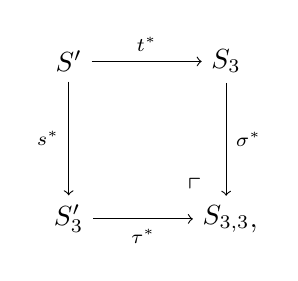
\begin{tikzpicture}
        \node (LT) at (0, 2) {$S'$}; 
	\node (RT) at (2, 2) {$S_3$}; 
        \node (LB) at (0, 0) {$S_3'$}; 
	\node (RB) at (2, 0) {$\s$}; 
	\node at (2.35, -0.125) {,}; 
	\node at (1.6, 0.4) {$\ulcorner$}; 
	\draw [->] (LT) -- node [above] {$\scriptstyle t^*$} (RT); 
	\draw [->] (LT) -- node [left] {$\scriptstyle s^*$} (LB); 
	\draw [->] (RT) -- node [right] {$\scriptstyle \sigma^*$} (RB); 
	\draw [->] (LB) -- node [below] {$\scriptstyle \tau^*$} (RB); 
\end{tikzpicture}
\end{center}
where $s^*$ is the inclusion, and $t^*$ sends $a'$ to $r(a)$ (cf.\thinspace{P}roposition \ref{prop:isog}; 
the image of $\Delta'$ is automatically invertible in $S_3$ by construction of $C'$).  
Then $\sigma^*$ and $\tau^*$ classify the subgroup $G$ of $C$, and the subgroup $G'$ of $C'$, respectively.  
Via the canonical isomorphism 
\[
 \frac{C'}{G'} \cong \frac{C/G}{C[3]/G}, 
\]
the ring 
\[
 \s \cong S[\A,\A'] \Big/ \Big( \A^4 - 6 \A^2 + (a^2 - 8) \A - 3, (\A')^4 - 6 (\A')^2 + \big( r(a)^2 - 8 \big) \A' - 3 \Big) 
\]
carries the universal example of a chain $G < C[3]$ of subgroups of $C$ with $|G| = |C[3]/G| = 3$.  

\begin{prop}
\label{prop:-p}
 The following diagram of elliptic curves over $\s$ commutes: 
 \begin{center}
 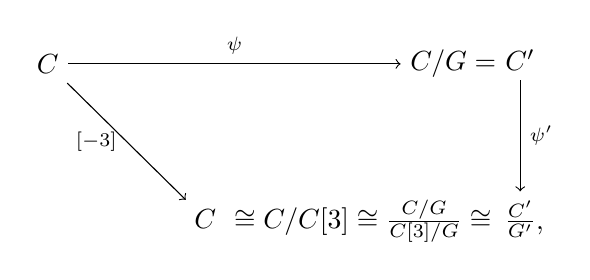
\begin{tikzpicture}
         \node (LT) at (0, 2) {$C$}; 
         \node (MT) at (5.15, 2) {$C/G = $}; 
         \node (RT) at (6, 2.05) {$C'$}; 
         \node (LB) at (2, 0.03) {$C$}; 
         \node (MB) at (4, 0) {$ \cong C/C[3] \cong \frac{C/G}{C[3]/G} \cong $}; 
         \node (RB) at (6, 0.025) {$\frac{C'}{G'}$}; 
         \node at (6.25, -0.125) {,}; 
         \draw [->] (LT) -- node [above] {$\scriptstyle \psi$} (MT); 
         \draw [->] (LT) -- node [left] {$\scriptstyle [-3]$} (LB); 
         \draw [->] (RT) -- node [right] {$\scriptstyle \psi'$} (RB); 
 \end{tikzpicture}
 \end{center}
 where the isomorphisms in the bottom row are the canonical ones.  
\end{prop}
\begin{proof}
 As noted in Remark \ref{rmk:lubin}, both $\psi$ and $\psi'$ restrict to the supersingular locus over $\BF_9$ as the third-power Frobenius endomorphism $\psi_0$.  
 By Honda--Tate theory, $\psi_0$ satisfies 
 \[
  \psi_0^2 + 3 = 0,~~~~\text{or}~~~~\psi_0^2 + 3 \psi_0 + 3 = 0,~~~~\text{or}~~~~\psi_0^2 - 3 \psi_0 + 3 = 0 
 \]
 in the endomorphism ring of the supersingular elliptic curve.  
 We can exclude the latter two possibilities by checking the action of $\psi_0$ at a specific 2-torsion point $(-1,0)$ of the supersingular elliptic curve 
 \[
  y^2 + 2 i x y + 2 i y = x^3 + x^2 
 \]
 over $\BF_9$, where $i$ is an element generating $\BF_9$ over $\BF_3$ with $i^2 = -1$ (cf.\thinspace\eqref{h}).  
 It remains to show that $\psi_0^2 = [-3]$ over $\BF_9$ lifts to 
 \[
  \psi' \circ \psi = [-3] \co C \to C'/G' 
 \]
 over $\s$, where by abuse of notation $[-3]$ denotes the map $[-3]$ on $C$ composed with the canonical isomorphisms from $C$ to $C'/G'$.  
 
 Consider the commutative diagram 
 \begin{center}
 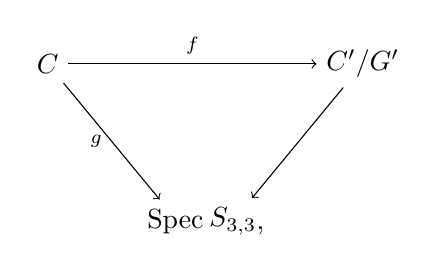
\begin{tikzpicture}
         \node (LT) at (0, 2) {$C$}; 
         \node (RT) at (4, 2) {$C'/G'$}; 
         \node (MB1) at (1.65, 0) {$\Spec$}; 
         \node (MB2) at (2.35, 0) {$\s$}; 
         \node at (2.7, -0.125) {,}; 
         \draw [->] (LT) -- node [above] {$\scriptstyle f$} (RT); 
         \draw [->] (LT) -- node [left] {$\scriptstyle g$} (MB1); 
         \draw [->] (RT) -- (MB2); 
 \end{tikzpicture}
 \end{center}
 where $f$ denotes $\psi' \circ \psi - [-3]$, and $g$ is the structure morphism of $C$ over $\s$.  Let 
 \[
  \Sigma = \{ s \in \Spec \s~|~~f_s \co C_s \to (C'/G')_s ~\text{is zero} \}, 
 \]
 where $(-)_s$ denotes the fiber of the structure morphism over $s$ 
 (and we will similarly use $(-)_U$ to denote the restriction over an open subscheme $U$ of the base scheme $\Spec \s$).  
 By considering the supersingular locus, we have seen that $\Sigma$ is nonempty, and we want to show that $\Sigma = \Spec \s$.  
 Since $\Spec \s$ is connected, we need only show that $\Sigma$ is both open and closed.  

 To see that $\Sigma$ is open, we take $s \in \Sigma$ and show that $f_U = 0$ for some open neighborhood $U$ of $s$.  
 Let $V$ be an affine open neighborhood of the identity of $C'/G'$, disjoint from the closed subscheme $(C'/G')[2]^\times$ of points of ``exact order 2''.  
 Then $f^{-1}(V)$ is an open subscheme of $C$ containing $C_s$.  
 Since $g$ is proper, it is closed, and thus $f^{-1}(V)$ contains $g^{-1}(U)$ for some affine open neighborhood $U$ of $s$ in $\Spec \s$.  
 Now $f_U \co C_U \to C'/G'$ factors through $V$, and we want to show that $f_U = 0$.  
 Since $V$ is affine, $f_U \co C_U \to V$ factors through $\Spec \G(C_U, \CO_{C_U})$.  
 Since $g$ is proper, smooth and surjective with geometrically connected fibers, there is an isomorphism 
 \[
  \CO_{\Spec \s} \stackrel{\cong}{\longrightarrow} g_*\CO_C 
 \]
 of formation compatible with arbitrary base change; in particular, $\Spec \G(C_U, \CO_{C_U}) \cong U$.  
 Thus $f_U$ factors as 
 \[
  C_U \stackrel{g}{\longrightarrow} U \stackrel{h}{\longrightarrow} V \subset (C'/G'), 
 \]
 where $h$ is a section of $(C'/G')_U$.  
 Since $f_U$ is a morphism of group schemes, $h$ is fixed by $[-1]$, and is hence the identity, as $V$ is disjoint from $(C'/G')[2]^\times$.  
 Thus $f_U = 0$.  

 To see that $\Sigma$ is closed, note that the inverse image in $C$ of the identity of $C'/G'$ is a closed subscheme of $C$, since $C'/G'$ is separated.  
 Thus its complement $W \subset C$ is open.  
 Since $g$ is flat and of finite presentation, it is open, and thus $g(W)$ is open in $\Spec \s$.  
 As its complement, $\Sigma$ is then closed.  
\end{proof}

\begin{cor}
\label{cor:-p}
 The following relations hold in $\s$: 
 \[
  \A \A' + 3 = 0, 
 \]
 and 
 \[
  \A' = -\A^3 + 6 \A + (-a^2 + 8).  
 \]
\end{cor}
\begin{proof}
 The isogenies in the diagram in Proposition \ref{prop:-p} induce maps on relative cotangent spaces at the identity, 
 and by Proposition \ref{prop:isog} we have a commutative diagram 
 \begin{center}
 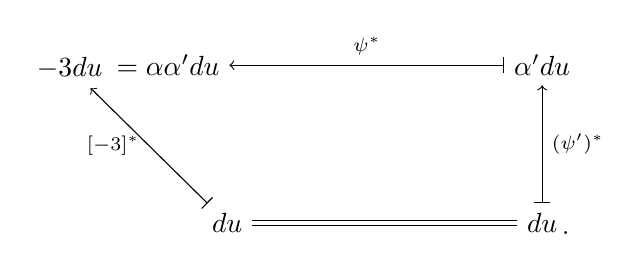
\begin{tikzpicture}
         \node (LT) at (0, 1.97) {$-3 du$}; 
         \node (MT) at (1.25, 2) {$= \A \A' du$}; 
         \node (RT) at (6, 2) {$\A' du$}; 
         \node (LB) at (2, 0) {$du$}; 
         \node (RB) at (6, 0) {$du$}; 
         \node at (6.3, -0.125) {.}; 
         \draw [|->] (RT) -- node [above] {$\scriptstyle \psi^*$} (MT); 
         \draw [|->] (LB) -- node [left] {$\scriptstyle [-3]^*$} (LT); 
         \draw [|->] (RB) -- node [right] {$\scriptstyle (\psi')^*$} (RT); 
         \draw [double distance=1.3pt] (LB) -- (RB); 
 \end{tikzpicture}
 \end{center}
 The first stated relation is read off from above.  From this and $w(\A) = 0$, we then get the second relation.  
\end{proof}
\begin{rmk}
 As noted in Remark \ref{rmk:alpha}, the analog of $\A$ at the prime 2 coincides with the parameter $d$ used in \cite[Section 3]{h2p2}.  
 Thus, with the notations there, $d$ and $d'$ satisfy an analogous relation $d d' + 2 = 0$ in the ring $S_{2,2}$.  
\end{rmk}

Let $S_9$ be the pullback in the diagram of commutative rings 
\begin{equation}
\label{S9}
 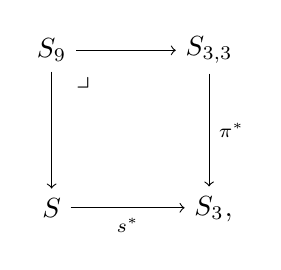
\begin{tikzpicture}[baseline=(current bounding box.center)]
         \node (LT) at (0, 2) {$S_9$}; 
         \node (RT) at (2, 2) {$\s$}; 
         \node (LB) at (0, 0) {$S$}; 
         \node (RB) at (2, 0) {$S_3$}; 
         \node at (2.25, -0.125) {,}; 
         \node at (0.4, 1.6) {$\lrcorner$}; 
         \draw [->] (LT) --  (RT); 
         \draw [->] (LT) --  (LB); 
         \draw [->] (RT) -- node [right] {$\scriptstyle \pi^*$} (RB); 
         \draw [->] (LB) -- node [below] {$\scriptstyle s^*$} (RB); 
 \end{tikzpicture}
\end{equation}
where $s^*$ is again the inclusion, and $\pi^*$ sends $a$ to $a$, $\A$ to $\A$, $a'$ to $r(a)$, and $\A'$ to $-\A^3 + 6 \A + (-a^2 + 8)$ as in Corollary \ref{cor:-p}.  
The map $\pi^*$ classifies the chain of subgroups $G < C[3]$ in $C$.  
Thus the universal example of an order-9 subgroup of $C$ is defined over $S_9$, and the map $S_9 \to S$ classifies $C[3]$.  

Equipped with the geometry above, we now turn to power operations.  

Let $A$ be a $K(2)$-local commutative $E$-algebra.  
From the total power operation on $E_0$ in Section \ref{sec:psi}, we have a total power operation 
\[
 \p \co A_0 \to A_0 \otimes_{E_0} (E^0 B\Sigma_3 / I) \cong A_0 [\A] \big/ \big( w(\A) \big), 
\]
With the notations in \eqref{w'}, we also have a composite of total power operations 
\[
 \p \circ \p \co A_0 \to \big( A_0 \otimes_{E_0} (E^0 B\Sigma_3 / I) \big) \tensor[^\p]{\otimes}{_{E_0}} (E^0 B\Sigma_3 / I) 
\]
\[
 ~~~~~~~~~~~~~~~~~~~~~~~~~~~~~~~~~~~~~~~~\cong \Big( A_0 [\A'] \big/ \big( w'(\A') \big) \Big) \tensor[^\p]{\otimes}{_{E_0}} \Big( E^0 [\A] \big/ \big( w(\A) \big) \Big), 
\]
where elements in $M \tensor[^\p]{\otimes}{_{E_0}} N$ are subject to the equivalence relation 
\[
 m \otimes (r \cdot n) \sim \big( m \cdot \p(r) \big) \otimes n
\]
for $m \in M$, $n \in N$, and $r \in E_0$, and 
\[
 \A' = \p(\A) = -\A^3 + 6 \A + (-h + 12)
\]
by Corollary \ref{cor:-p}.  

Define the {\em individual power operations} 
\[
 Q_i \co A_0 \to A_0, 
\]
for $i = 0, 1, 2, 3$, by 
\[
 \p (x) = Q_0(x) + Q_1(x) \A + Q_2(x) \A^2 + Q_3(x) \A^3.  
\]

\begin{prop}
\label{prop:Gamma}
 The following relations hold among the individual power operations $Q_0$, $Q_1$, $Q_2$, and $Q_3$: 
 \begin{enumerate}[(i)]
  \item Additivity 

  $Q_i(x+y) = Q_i(x) + Q_i(y)$; 

  \item Action on scalars 
  
  $Q_0(1) = 1$, 

  $Q_1(1) = Q_2(1) = Q_3(1) = 0$, 

  $Q_0(h) = h^3 - 36 h^2 + 390 h - 1212$, 

  $Q_1(h) = -6 h^2 + 144 h - 712$, 

  $Q_2(h) = 3 h - 36$, 

  $Q_3(h) = h^2 - 24 h + 120$, 

  $Q_0(a) = a^3 - 12 a + 12 a^{-1}$, 

  $Q_1(a) = -6 a + 20 a^{-1}$, 

  $Q_2(a) = 4 a^{-1}$, 

  $Q_3(a) = a - 4 a^{-1}$; 

  \item Commutation relations 

  $Q_0(h x) = (h^3 - 36 h^2 + 390 h - 1212) Q_0(x) + (3 h^2 - 72 h + 360) Q_1(x) + (9 h - 108) Q_2(x) + 24 Q_3(x)$, 

  $Q_1(h x) = (-6 h^2 + 144 h - 712) Q_0(x) + (-18 h + 228) Q_1(x) + (-72) Q_2(x) + (h - 12) Q_3(x)$, 

  $Q_2(h x) = (3 h - 36) Q_0(x) + 8 Q_1(x) + 12 Q_2(x) + (-24) Q_3(x)$, 

  $Q_3(h x) = (h^2 - 24 h + 120) Q_0(x) + (3 h - 36) Q_1(x) + 8 Q_2(x) + 12 Q_3(x)$, 

  $Q_0(a x) = (a^3 - 12 a + 12 a^{-1}) Q_0(x) + (3 a - 12 a^{-1}) Q_1(x) + (12 a^{-1}) Q_2(x) + (-12 a^{-1}) Q_3(x)$, 

  $Q_1(a x) = (-6 a + 20 a^{-1}) Q_0(x) + (-20 a^{-1}) Q_1(x) + (- a + 20 a^{-1}) Q_2(x) + (4 a - 20 a^{-1}) Q_3(x)$, 

  $Q_2(a x) = (4 a^{-1}) Q_0(x) + (-4 a^{-1}) Q_1(x) + (4 a^{-1}) Q_2(x) + (- a - 4 a^{-1}) Q_3(x)$, 

  $Q_3(a x) = (a - 4 a^{-1}) Q_0(x) + (4 a^{-1}) Q_1(x) + (-4 a^{-1}) Q_2(x) + (4 a^{-1}) Q_3(x)$; 

  \item Adem relations 

  $Q_1Q_0(x) = (-6) Q_0Q_1(x) + (6 h - 72) Q_0Q_2(x) + (-6 h^2 + 144 h - 747) Q_0Q_3(x) + 18 Q_1Q_2(x) + 3 Q_2Q_1(x) + (-18 h + 216) Q_1Q_3(x) + (-54) Q_2Q_3(x) + (-9) Q_3Q_2(x)$, 

  $Q_2Q_0(x) = (-3) Q_0Q_2(x) + (3 h - 36) Q_0Q_3(x) + 9 Q_1Q_3(x) + 3 Q_3Q_1(x)$, 

  $Q_3Q_0(x) = Q_0Q_1(x) + (-h + 12) Q_0Q_2(x) + (h^2 - 24 h + 126) Q_0Q_3(x) + (-3) Q_1Q_2(x) + (3 h - 36) Q_1Q_3(x) + 9 Q_2Q_3(x)$; 

  \item Cartan formulas 

  $Q_0(xy) = Q_0(x) Q_0(y) + 3 \big(Q_1(x) Q_3(y) + Q_2(x) Q_2(y) + Q_3(x) Q_1(y)\big) + 18 Q_3(x) Q_3(y)$, 

  $Q_1(xy) = \big(Q_0(x) Q_1(y) + Q_1(x) Q_0(y)\big) + (-h + 12) \big(Q_1(x) Q_3(y) + Q_2(x) Q_2(y) + Q_3(x) Q_1(y)\big) + 3 \big(Q_2(x) Q_3(y) + Q_3(x) Q_2(y)\big) + (-6h + 72) Q_3(x) Q_3(y)$, 

  $Q_2(xy) = \big(Q_0(x) Q_2(y) + Q_1(x) Q_1(y) + Q_2(x) Q_0(y)\big) + 6 \big(Q_1(x) Q_3(y) + Q_2(x) Q_2(y) + Q_3(x) Q_1(y)\big) + (-h + 12) \big(Q_2(x) Q_3(y) + Q_3(x) Q_2(y)\big) + 39 Q_3(x) Q_3(y)$, 

  $Q_3(xy) = \big(Q_0(x) Q_3(y) + Q_1(x) Q_2(y) + Q_2(x) Q_1(y) + Q_3(x) Q_0(y)\big) + 6 \big(Q_2(x) Q_3(y) + Q_3(x) Q_2(y)\big) + (-h + 12) Q_3(x) Q_3(y)$; 

  \item Frobenius congruence 

  $Q_0(x) \equiv x^3 \md 3$, with $\theta \co A_0 \to A_0$ such that $Q_0(x) = x^3 + 3 \theta(x)$.  
 \end{enumerate}
\end{prop}
\begin{proof}
 Except for (iv), all the relations can be derived directly from the formulas in Corollary \ref{cor:psi3} and the fact that $\p$ is a ring homomorphism.  

 Write $\HS'$, $\HS_3'$, $\HS_{3,3}$, and $\HS_9$, analogous to $\HS_3$ in \eqref{S3hat}, to denote the completions of rings.  
 In view of \eqref{S9} and the moduli interpretations of $\s$ and $S_9$, we note that the composite 
 \[
  A_0 \stackrel{\p}{\longrightarrow} A_0 \tensor[]{\otimes}{_{\HS}^{s^*}} \HS_3 
  \stackrel{\p}{\longrightarrow} A_0 \tensor[]{\otimes}{_{\HS'}^{s^*}} \HS_3' \tensor[^{t^*}]{\otimes}{_{\HS}^{s^*}} \HS_3 
  \cong A_0 \tensor[]{\otimes}{_{\HS}^{s^*}} \HS_{3,3} 
 \]
 factors through $A_0 \otimes_{\HS} \HS_9$.  In terms of formulas, we have 
 \begin{eqnarray*}
  \p \big( \p(x) \big) & = & \p \big( Q_0(x) + Q_1(x) \A + Q_2(x) \A^2 + Q_3(x) \A^3 \big) \\
                       & = & \p \big( Q_0(x) \big) + \p \big( Q_1(x) \big) \A' + \p \big( Q_2(x) \big) (\A')^2 + \p \big( Q_3(x) \big) (\A')^3 \\
                       & = & \sum_{i,~j~=~0}^3 Q_iQ_j(x) \A^i \big( -\A^3 + 6 \A + (-h + 12) \big)^j, 
 \end{eqnarray*}
 where the last expression is the projection to $\HS_3$ from $\HS_{3,3}$ along $\pi^*$.  
 Factoring through $A_0 \otimes_{\HS} \HS_9$ then means that the coefficients of $\A$, $\A^2$, and $\A^3$ in this last expression must be 0 
 ($\A$ satisfies a quartic equation in $\HS_3$).  This gives the three relations in (iv).
\end{proof}

\begin{defn}
\label{def}
 We define an associative ring $\G$ equipped with a ring homomorphism $\eta \co \HS \to \G$ as follows 
 \footnote{For any element $s \in \HS = E_0$, $\eta(s)$ corresponds to the multiplication-by-$s$ operation on the $E_0$-algebra $A_0$ (\cff{Section 6}{cong}).  }.  
 The ring $\G$ is generated over $\HS$ via $\eta$ by elements $Q_0$, $Q_1$, $Q_2$, and $Q_3$, subject to {\em commutation relations} and {\em Adem relations}.  
 The commutation relations state that the $Q_i$'s commute with elements of $\BZ_9 \subset \HS$, and that 

 $Q_0 h = (h^3 - 36 h^2 + 390 h - 1212) Q_0 + (3 h^2 - 72 h + 360) Q_1 + (9 h - 108) Q_2 + 24 Q_3$, 

 $Q_1 h = (-6 h^2 + 144 h - 712) Q_0 + (-18 h + 228) Q_1 + (-72) Q_2 + (h - 12) Q_3$, 

 $Q_2 h = (3 h - 36) Q_0 + 8 Q_1 + 12 Q_2 + (-24) Q_3$, 

 $Q_3 h = (h^2 - 24 h + 120) Q_0 + (3 h - 36) Q_1 + 8 Q_2 + 12 Q_3$.  

 The Adem relations are 

 $Q_1Q_0 = (-6) Q_0Q_1 + (6 h - 72) Q_0Q_2 + (-6 h^2 + 144 h - 747) Q_0Q_3 + 18 Q_1Q_2 + 3 Q_2Q_1 + (-18 h + 216) Q_1Q_3 + (-54) Q_2Q_3 + (-9) Q_3Q_2$, 

 $Q_2Q_0 = (-3) Q_0Q_2 + (3 h - 36) Q_0Q_3 + 9 Q_1Q_3 + 3 Q_3Q_1$, 

 $Q_3Q_0 = Q_0Q_1 + (-h + 12) Q_0Q_2 + (h^2 - 24 h + 126) Q_0Q_3 + (-3) Q_1Q_2 + (3 h - 36) Q_1Q_3 + 9 Q_2Q_3$.  
\end{defn}

\begin{rmk}
\label{rmk:rank}
 Proposition \ref{prop:Gamma} describes explicitly the structure of $\G$ as a {\em graded twisted bialgebra} over $E_0 = \HS$ (\cff{Section 5}{cong} and \cite[2.1]{h2p2}).  
 In particular it follows using commutation relations and Adem relations that $\G$ has an {\em admissible basis}.  
 That is, it is free as a left $\HS$-module on the elements of the form 
 \[
  Q_0^i Q_{k_1} \cdots Q_{k_r}, 
 \]
 where $i, r \geq 0$, and $k_j = 1, 2,$ or 3.  
 Note that if we write $\G[d]$ for the degree-$d$ part of $\G$, then $\G[d]$ is of rank $1 + 3 + \cdots + 3^d$.  
\end{rmk}

\begin{exam}
\label{ex:omega}
 We have $E^0 S^2 \cong \BZ_9 \llbracket h \rrbracket [u] / (u^2)$.  
 By definition of $\A$ in \eqref{u'v'}, the $Q_i$'s act canonically on $E^0 S^2$: 
 \[
  Q_i \cdot u = \left\{
  \begin{array}{ll}
    u,  & \quad \text{if $i = 1$, }\\
    0,  & \quad \text{if $i \neq 1$.  }\\
  \end{array}
  \right.
 \]
 Let $\omega$ be the kernel of $E^0 S^2 \to E^0$.  It is a {\em $\G$-module} (\cff{2.2}{h2p2}) on one generator $u$, and its $\G$-module structure is canonical as above.  
\end{exam}

Following the terminology in \cite[Section 2]{cong} and \cite[2.5 and 2.6]{h2p2}, we can now describe the power operation structure on $K(2)$-local commutative $E$-algebras.  
\begin{thm}
\label{thm}
 Let $A$ be a $K(2)$-local commutative $E$-algebra.  
 Let $\G$ be the graded twisted bialgebra over $E_0$ given in Definition \ref{def}, and let $\omega$ be the $\G$-module given in Example \ref{ex:omega}.  
 Then $A_*$ is an {\em $\omega$-twisted $\BZ/2$-graded amplified $\G$-ring}.  In particular, 
 \[
  \pi_* L_{K(2)} \BP_E (\Sigma^d E) ~ \cong ~ \big( F_d \big)_{(3,h)}^\wedge ~ , 
 \]
 where $F_d$ is the free $\omega$-twisted $\BZ/2$-graded amplified $\G$-ring on one generator in degree $d$.  
\end{thm}
Formulas of $\G$ aside, this result is essentially due to Rezk \cite{cong, h2p2}.  
\begin{proof}
 Let $\TG$ be the graded twisted bialgebra of power operations on $E$ described in \cite[Section 6]{cong}.  
 It suffices to identify $\TG$ with $\G$.  
 There is a direct sum decomposition $\TG = \bigoplus_{d \geq 0} \TG[d]$, where the pieces come from the $E$-homology of $B\Sigma_{3^d}$ (\cff{6.2}{cong}).  
 There is a degree-preserving ring homomorphism $\phi \co \G \to \TG$ which is an isomorphism in degrees 0 and 1 (cf.\thinspace{C}orollary \ref{cor:psi3}).  
 Since $\TG$ is generated in degree 1 by a transfer argument, $\phi$ is surjective.  
 Since $\G[d]$ and $\TG[d]$ are of the same rank $1 + 3 + \cdots + 3^d$ as free modules over $E_0$ by Remark \ref{rmk:rank} and \cite[Theorem 1.1]{Str98}), 
 $\phi$ is also injective.  
\end{proof}


\section{$K(1)$-local power operations}
\label{sec:K(1)}

Let $F = L_{K(1)} E$.  The general pattern of the relationship between $K(1)$-local power operations and the power operations in Section \ref{sec:psi} is as follows: 
\begin{center}
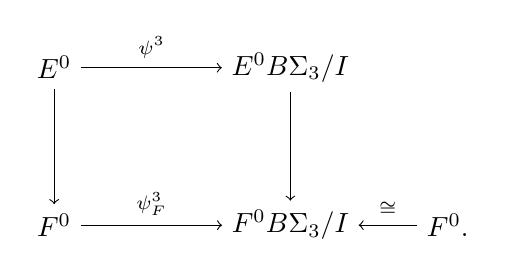
\begin{tikzpicture}
        \node (LT) at (0, 2) {$E^0$}; 
        \node (RT) at (3, 2) {$E^0 B\Sigma_3 / I$}; 
        \node (LB) at (0, 0) {$F^0$}; 
        \node (MB) at (3, 0) {$F^0 B\Sigma_3 / I$}; 
        \node (RB) at (5, 0) {$F^0.$}; 
        \draw [->] (LT) -- node [above] {$\scriptstyle \p$} (RT); 
        \draw [->] (LT) -- (LB); 
        \draw [->] (RT) -- (MB); 
        \draw [->] (LB) -- node [above] {$\scriptstyle \psi_F^3$} (MB); 
        \draw [->] (RB) -- node [above] {$\scriptstyle \cong$} (MB); 
\end{tikzpicture}
\end{center}
Recall from Proposition \ref{prop:isog} and Corollary \ref{cor:psi3} that $\p$ arises from the universal degree-3 isogeny 
which is parametrized by the ring $S_3$ with 
\[
 \HS_3 = \big( S_3 \big)_{(3,h)}^\wedge \cong E^0 B\Sigma_3 / I.  
\]
The vertical maps are induced by the $K(1)$-localization $E \to F$.  In terms of 
homotopy groups, this is obtained by inverting the generator $h$ (so that 
the resulting formal group is of height at most 1) and completing at the ideal 
$(3)$: 
\[
 E_* = \BZ_9 \llbracket h \rrbracket [u^{\pm1}]~~~~~~~~\text{and}~~~~~~~~F_* = \BZ_9 \llbracket h \rrbracket [h^{-1}]_3^\wedge [u^{\pm1}].  
\]
Explicitly, 
\begin{equation}
\label{explicit}
 F_0 = \BZ_9 (\!(h)\!)_3^\wedge = \varprojlim_k \BZ_9 (\!(h)\!) /(3^k) = 
 \left.\left\{\sum_{n = -\infty}^{\infty} c_n h^n~\right|~c_n \in \BZ_9, 
 \lim_{n \to -\infty} c_n = 0\right\}.  
\end{equation}
The formal group $\HC$ over $E^0$ has a unique order-3 subgroup after being pulled back to $F^0$ (cf.\thinspace{R}emark \ref{rmk:dmod3}), 
and the composite map 
\[
 E^0 B\Sigma_3 / I \to F^0 B\Sigma_3 / I \cong F^0 
\]
classifies this subgroup.  
The map 
\[
 E^0 B\Sigma_3 / I \to F^0 B\Sigma_3 / I 
\]
factors through $F^0 \otimes_{E^0} E^0 B\Sigma_3 / I$; along the base change 
\[
 E^0 B\Sigma_3 / I \to F^0 \otimes_{E^0} E^0 B\Sigma_3 / I, 
\]
the special fiber of the 3-divisible group $\HC$ which consists solely of a formal component may split into formal and \'etale components.  
We want to take the formal component so as to keep track of the unique order-3 subgroup of the formal group over $F^0$ 
which gives rise to the $K(1)$-local power operation $\psi_F^3$.  

As in Proposition \ref{prop:isog}, the ring 
\[
 S_3 = S[\A] \big/ \big( w(\A) \big) 
\]
parametrizes order-3 subgroups of $C$.  Since 
\[
 w(\A) = \A^4 - 6 \A^2 + (h - 12) \A - 3 \equiv \A (\A^3 + h) \md 3, 
\]
the equation $w(\A) = 0$ has a unique root $\A = 0$ in $\BF_3 (\!(h)\!)$ (in view of \eqref{explicit}, $\A^3 + h$ cannot be zero).  
By Hensel's Lemma this unique root lifts to a root in $\BZ_9 (\!(h)\!)_3^\wedge$; 
it corresponds to the unique order-3 subgroup of $\HC$ over $F^0 = \BZ_9 (\!(h)\!)_3^\wedge$.  
Plugging this specific value of $\A$ into the formulas of 
\[
 \p \co E^0 \to E^0 [\A] \big/ \big( w(\A) \big) 
\]
given in Corollary \ref{cor:psi3}, we then get an endomorphism of the ring $F^0$.  
This endomorphism is the $K(1)$-local power operation $\psi_F^3$.  

Explicitly, with $h$ invertible in $F^0$, we can solve for $\A$ from the equation $w(\A) = 0$ by first writing 
\[
 \A = \frac{1}{h - 12} (3 + 6 \A^2 - \A^4) = (3 + 6 \A^2 - \A^4) \cdot \sum_{n = 1}^\infty 12^{n-1} h^{-n} 
\]
and then substituting $\A$ recursively.  We plug this into $\p(h)$ and get 
\[
 \psi_F^3(h) = h^3 - 36 h^2 + 372 h - 996 + 186 h^{-1} + 2232 h^{-2} + \cdots.  
\]
Similarly we have 
\[
 \psi_F^3(a) = a^3 - 12 a - 6 a^{-1} - 84 a^{-3} - 933 a^{-5} - 10956 a^{-7} + \cdots.  
\]


\appendix
\section*{Appendices}

The calculations in this paper involve power series expansions and basic manipulations of long polynomials with large coefficients, 
namely division, factorization, and finding greatest common divisors.  
These are done using the software {\em Wolfram Mathematica 8}.  
In particular the commands \texttt{Reduce} and \texttt{Solve} are used to extract relations out of given identities.


\section{List of formulas in the proof of Proposition \ref{prop:tors}}
\label{apx:tors}

$\Tf(u) = -u^4 (-3 - 3 a u + 8 u^2 - a^2 u^2 + 9 a u^3 - 6 u^4 + 6 a^2 u^4 + 
    7 a u^5 + a^3 u^5 + 3 a^2 u^6 + 3 a u^7 + u^8) / a^2$

$Q_1(v) = \frac{1}{a} - d - \frac{2 d^2}{a} + a d^2 + 2 d^3 + \frac{d^4}{a} + (-1 + 2 a d + d^2) v + 
 a v^2$

$R_1(v) = \frac{d^3}{a} + 2 d^4 - \frac{2 d^5}{a} + a d^5 + 
 2 d^6 + \frac{d^7}{a} + (-\frac{1}{a} + \frac{3 d^2}{a} + 2 d^3 - \frac{3 d^4}{a} + a d^4 + 
    2 d^5 + \frac{d^6}{a}) v$

$Q_2(v) = -a (1 + a d - 4 d^2 - 4 a d^3 + 6 d^4 - a^2 d^4 + a d^5 - 4 d^6 + 
    a^2 d^6 + 2 a d^7 + d^8 + a v - 3 a d^2 v - 2 a^2 d^3 v + 
    3 a d^4 v - a^3 d^4 v - 2 a^2 d^5 v - a d^6 v) / (-1 + 3 d^2 + 
   2 a d^3 - 3 d^4 + a^2 d^4 + 2 a d^5 + d^6)^2$

$R_2 = -a d^4 (-3 - 3 a d + 8 d^2 - a^2 d^2 + 9 a d^3 - 6 d^4 + 
    6 a^2 d^4 + 7 a d^5 + a^3 d^5 + 3 a^2 d^6 + 3 a d^7 + d^8) / (-1 + 
   3 d^2 + 2 a d^3 - 3 d^4 + a^2 d^4 + 2 a d^5 + d^6)^2$

$S(d) = \frac{d^3}{a} + 2 d^4 - \frac{2 d^5}{a} + a d^5 + 
 2 d^6 + \frac{d^7}{a}$

$T(d) = -\frac{1}{a} + \frac{3 d^2}{a} + 2 d^3 - \frac{3 d^4}{a} + a d^4 + 
    2 d^5 + \frac{d^6}{a}$

$M(u) = (-4096 a^6 + 13568 a^8 - 2672 a^{10} + 179 a^{12} - 
  4 a^{14} - 98304 a^7 u + 19456 a^9 u - 1280 a^{11} u + 28 a^{13} u + 
  8192 a^6 u^2 - 69120 a^8 u^2 + 17248 a^{10} u^2 - 1610 a^{12} u^2 + 
  66 a^{14} u^2 - a^{16} u^2 + 77824 a^7 u^3 - 41984 a^9 u^3 + 
  6384 a^{11} u^3 - 382 a^{13} u^3 + 8 a^{15} u^3 - 4096 a^6 u^4 - 
  55040 a^8 u^4 + 11792 a^{10} u^4 - 825 a^{12} u^4 + 19 a^{14} u^4 - 
  28672 a^7 u^5 + 6144 a^9 u^5 - 432 a^{11} u^5 + 10 a^{13} u^5) / (65536 a^8 - 16384 a^{10} + 1536 a^{12} - 
 64 a^{14} + a^{16})$

$N(u) = a (12288 a^6 - 106240 a^8 + 24400 a^{10} - 2073 a^{12} + 
   76 a^{14} - a^{16} + 307200 a^7 u - 99072 a^9 u + 11856 a^{11} u - 
   621 a^{13} u + 12 a^{15} u - 20480 a^6 u^2 + 296192 a^8 u^2 - 
   71856 a^{10} u^2 + 6555 a^{12} u^2 - 265 a^{14} u^2 + 4 a^{16} u^2 - 
   135168 a^7 u^3 + 199680 a^9 u^3 - 40272 a^{11} u^3 + 3082 a^{13} u^3 - 
   98 a^{15} u^3 + a^{17} u^3 + 4096 a^6 u^4 + 213760 a^8 u^4 - 
   22928 a^{10} u^4 - 1435 a^{12} u^4 + 239 a^{14} u^4 - 7 a^{16} u^4 + 
   12288 a^7 u^5 + 78592 a^9 u^5 - 16880 a^{11} u^5 + 1177 a^{13} u^5 - 
   27 a^{15} u^5 + 4096 a^6 u^6 + 83712 a^8 u^6 - 17936 a^{10} u^6 + 
   1257 a^{12} u^6 - 29 a^{14} u^6 + 28672 a^7 u^7 - 6144 a^9 u^7 + 
   432 a^{11} u^7 - 10 a^{13} u^7) / (65536 a^8 - 16384 a^{10} + 1536 a^{12} - 
 64 a^{14} + a^{16})$


\section{List of formulas in the proof of Proposition \ref{prop:isog}}
\label{apx:isog}

$v = u^3 - a u^4 + (1 + a^2) u^5 - 
 a (3 + a^2) u^6 + (1 + 6 a^2 + a^4) u^7 - 
 a (6 + 10 a^2 + a^4) u^8 + (1 + 20 a^2 + 15 a^4 + a^6) u^9 + O(u^{10})$

The group law on $C$ satisfies: 
\begin{itemize}
 \item given $P(u,v)$, the coordinates of $-P$ are 
 \[
  u_0 = -\frac{v}{u (u + v)}~~~~~~~~\text{and}~~~~~~~~v_0 = -\frac{v^2}{u^2 (u + v)}; 
 \]

 \item given $P_1(u_1,v_1)$ and $P_2(u_2,v_2)$, the coordinates of $-(P_1 + P_2)$ are 
 \[
  u_3 = a k - \frac{b}{1 + k} - u_1 - u_2~~~~~~~~\text{and}~~~~~~~~v_3 = k u_3 + b, 
 \]
 where $k = \frac{v_1 - v_2}{u_1 - u_2}$ is the slope and $b = \frac{u_1 v_2 - u_2 v_1}{u_1 - u_2}$ is the $v$-intercept of the line through $P_1$ and $P_2$.  
\end{itemize}
Thus, given $P(u,v)$ and $Q(d,e)$, to compute formulas of $u\big(\psi(P)\big)$ and $v\big(\psi(P)\big)$, 
\begin{itemize}
 \item set 
 \[
  (u_1,v_1) = \left( -\frac{v}{u (u + v)},-\frac{v^2}{u^2 (u + v)} \right)~~~~~~~~\text{and}~~~~~~~~(u_2,v_2) = (d,e), 
 \]
 and take 
 \[
  P - Q = (u_3,v_3); 
 \]
 \item set 
 \[
  (u_1,v_1) = (u,v)~~~~~~~~\text{and}~~~~~~~~(u_2,v_2) = (d,e), 
 \]
 and take 
 \[
  P + Q = \left( -\frac{v_3}{u_3 (u_3 + v_3)},-\frac{v_3^2}{u_3^2 (u_3 + v_3)} \right).  
 \]
\end{itemize}
Plugging the coordinates of $P - Q$ and $P + Q$ into \eqref{defpsi}, and in view of $f(d) = 0$ as in Proposition \ref{prop:tors}, 
we have in \eqref{u'v'}, among coefficients of higher powers of $u$, 

$\A = -(-18 - 12 a d + 2 d^2 + a^2 d^2 - 15 a d^3 + 4 a^3 d^3 + 2 d^4 + 
  a^2 d^4 + a^4 d^4 - 6 a d^5 + 3 a^3 d^5 - 2 d^6 + 3 a^2 d^6 + a d^7) \big/ \big((-4 + a) (4 + a)\big)$, 

$\beta = -(-12 - 6 a^2 - 117 a d + 3 a^3 d + 20 d^2 - 153 a^2 d^2 + 
   10 a^4 d^2 + 31 a d^3 - 80 a^3 d^3 + 6 a^5 d^3 - 4 d^4 - 
   96 a^2 d^4 - 4 a^4 d^4 + a^6 d^4 - 15 a d^5 - 33 a^3 d^5 + 
   3 a^5 d^5 - 4 d^6 - 33 a^2 d^6 + 3 a^4 d^6 - 11 a d^7 + a^3 d^7) \big/ \big((-4 + a) a^2 (4 + a)\big)$.  

$\A^3 / \beta = -(4 - 4 a^2 + 9 a d - 3 a^3 d - 12 d^2 + 21 a^2 d^2 - a^4 d^2 - 
  15 a d^3 + 11 a^3 d^3 + 12 d^4 + 6 a^2 d^4 + 3 a^4 d^4 - 13 a d^5 + 
  9 a^3 d^5 - 4 d^6 + 9 a^2 d^6 + 3 a d^7) \big/ \big((-4 + a) (4 + a)\big)$


%\nocite{*}
%\bibliographystyle{amsalpha}
%\bibliography{p3}
%\end{document}

\newcommand{\MRn}[2]{\href{http://www.ams.org/mathscinet-getitem?mr=#1}{MR#1} #2}
\begin{thebibliography}

\bibitem[AHS01]{cube}
M.~Ando, M.~J. Hopkins, and N.~P. Strickland, \emph{Elliptic spectra, the
  {W}itten genus and the theorem of the cube}, Invent. Math. \textbf{146}
  (2001), no.~3, 595--687. \MRn{1869850}{(2002g:55009)}

\bibitem[BMMS86]{H_infty}
R.~R. Bruner, J.~P. May, J.~E. McClure, and M.~Steinberger, \emph{{$H\sb \infty
  $} ring spectra and their applications}, Lecture Notes in Mathematics, vol.
  1176, Springer-Verlag, Berlin, 1986. \MRn{836132}{(88e:55001)}

\bibitem[BW05]{BW}
James Borger and Ben Wieland, \emph{Plethystic algebra}, Adv. Math.
  \textbf{194} (2005), no.~2, 246--283. \MRn{2139914}{(2006i:13044)}

\bibitem[EKMM97]{EKMM}
A.~D. Elmendorf, I.~Kriz, M.~A. Mandell, and J.~P. May, \emph{Rings, modules,
  and algebras in stable homotopy theory}, Mathematical Surveys and Monographs,
  vol.~47, American Mathematical Society, Providence, RI, 1997, With an
  appendix by M. Cole. \MRn{1417719}{(97h:55006)}

\bibitem[Gre88]{blind}
J.~P.~C. Greenlees, \emph{How blind is your favourite cohomology theory?},
  Exposition. Math. \textbf{6} (1988), no.~3, 193--208. \MRn{949783}{(89j:55001)}

\bibitem[Lub67]{lubin67}
Jonathan Lubin, \emph{Finite subgroups and isogenies of one-parameter formal
  {L}ie groups}, Ann. of Math. (2) \textbf{85} (1967), 296--302. \MRn{0209287}{(35 \#189)}

\bibitem[Lub79]{lubin79}
Jonathan Lubin, \emph{Canonical subgroups of formal groups}, Trans. Amer. Math.
  Soc. \textbf{251} (1979), 103--127. \MRn{531971}{(80j:14039)}

\bibitem[Reza]{lpo}
Charles Rezk, \emph{Lectures on power operations}, available at
  \url{http://www.math.uiuc.edu/~rezk/power-operation-lectures.dvi}.

\bibitem[Rezb]{h2p2}
\bysame, \emph{Power operations for {M}orava ${E}$-theory of height 2 at the
  prime 2}, \href{http://arxiv.org/abs/0812.1320}{arXiv:0812.1320}.

\bibitem[Rez09]{cong}
\bysame, \emph{The congruence criterion for power operations in {M}orava
  {$E$}-theory}, Homology, Homotopy Appl. \textbf{11} (2009), no.~2, 327--379.
  \MRn{2591924}{(2011e:55021)}

\bibitem[Sil09]{AEC}
Joseph~H. Silverman, \emph{The arithmetic of elliptic curves}, second ed.,
  Graduate Texts in Mathematics, vol. 106, Springer, Dordrecht, 2009.
  \MRn{2514094}{(2010i:11005)}

\bibitem[Ste62]{steenrod}
N.~E. Steenrod, \emph{Cohomology operations}, Lectures by N. E. Steenrod
  written and revised by D. B. A. Epstein. Annals of Mathematics Studies, No.
  50, Princeton University Press, Princeton, N.J., 1962. \MRn{0145525}{(26
  \#3056)}

\bibitem[Str98]{Str98}
N.~P. Strickland, \emph{Morava {$E$}-theory of symmetric groups}, Topology
  \textbf{37} (1998), no.~4, 757--779. \MRn{1607736}{(99e:55008)}

\bibitem[Voe03]{V}
Vladimir Voevodsky, \emph{Reduced power operations in motivic cohomology},
  Publ. Math. Inst. Hautes \'Etudes Sci. (2003), no.~98, 1--57. \MRn{2031198}{(2005b:14038a)}

\end{thebibliography}
\end{document}